\documentclass{mcmthesis}
\mcmsetup{CTeX = true,   % 使用 CTeX 套装时,设置为 true
        tcn = 0000, problem = B,
        sheet = true, titleinsheet = true, keywordsinsheet = true,
        titlepage = false, abstract = true}
\usepackage{palatino}
\usepackage{lipsum}
\title{The \LaTeX{} Template for MCM Version \MCMversion}
\author{\small \href{http://www.latexstudio.net/}
  {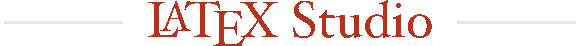
\includegraphics[width=7cm]{mcmthesis-logo}}}
\date{\today}
\begin{document}
\begin{abstract}
\lipsum[1]%写summary的地方
\begin{keywords}
keyword1; keyword2
\end{keywords}
\end{abstract}
\maketitle
\tableofcontents
\newpage

\section{Introduction}
\subsection{Background}

Lewis Mumford, a famous sociologist and literary critic,
once said in a metaphorical manner, ``Adding highway lanes
to deal with traffic congestion is like loosening your
belt to cure obesity.`` Fortunately, he did not experience
the worse congestion around today`s highway toll plaza.

Currently, with roaring number of vehicles, rising
construction costs and constrained available areas,
traffic jam becomes more and more serious but future
toll-plaza construction opportunities are limited to
improve this situation markedly. Figure 1 shows the
congestion in the toll plaza near Tappan Zee Bridge.

\begin{figure}[h]
\small
\centering
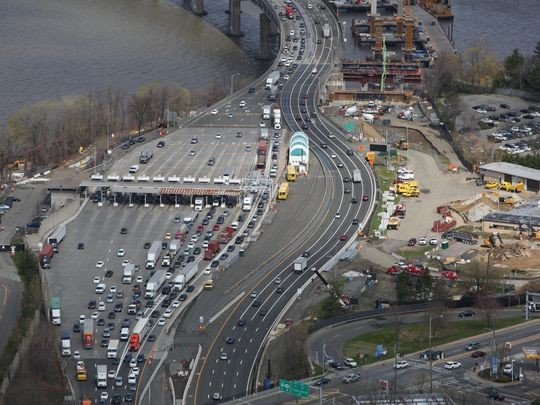
\includegraphics[width=10cm]{figure1}
\caption{Toll Plaza Congestion}\label{fig1}
\end{figure}

Subject to the constraints referred above, neither
increasing highway lanes nor building more tollbooths
seems practical enough to relieve traffic jam around a
toll plaza nowadays, particularly for some heavily-traveled
 roads such as the Garden State Parkway, New Jersey.
 Therefore, looking for some innovative design improvements
  on the geometric parameters of the extent toll plaza
  is an effective solution.


\subsection{Restatement of the Problem}
In this paper, we are required to explore if there is a
better-than-ever toll plaza model with specific shape,
size, and merging pattern. In this model, the prerequisite
is that vehicles fan in from $B$ tollbooth egress lanes down
to $L$ ($B\textgreater L$) lanes of traffic (i.e., the number of both
tollbooths and the lanes after merging are fixed). We aim
to construct a model that can optimize the arrangement
according to the following conditions.

\begin{itemize}
\item Enhance the capability of the accident prevention(A).
\item Maximize the throughput(T).
\item Minimize the cost of the land and road
construction(C).
\end{itemize}

Through our analysis, we determine if there are better
solutions than any toll plaza in common use. Afterwards,
the performance of our solution in light and heavy traffic
and other various situations along with corresponding
sensitivity analysis is discussed.

\subsection{Our Work}

\section{Assumptions}

\section{Notations}

\section{Model}
\subsection{Time Cost and Construction Cost}
\subsection{CA Model}

\section{Size}

\section{Shape}

\section{Merging Pattern}

Here, we devise a real-time merging control system for
toll plaza based on the precious work by M. Papageorgiou
et al. Through our improvement, it can be specially used
for the toll plaza we are discussing. In addition, this
system can effectively maximize the throughput by
maintaining the occupancy of departure area close to a
critical value. Figure \ref{fig2} illustrates the framework of
this system.

\begin{figure}[h]
\small
\centering
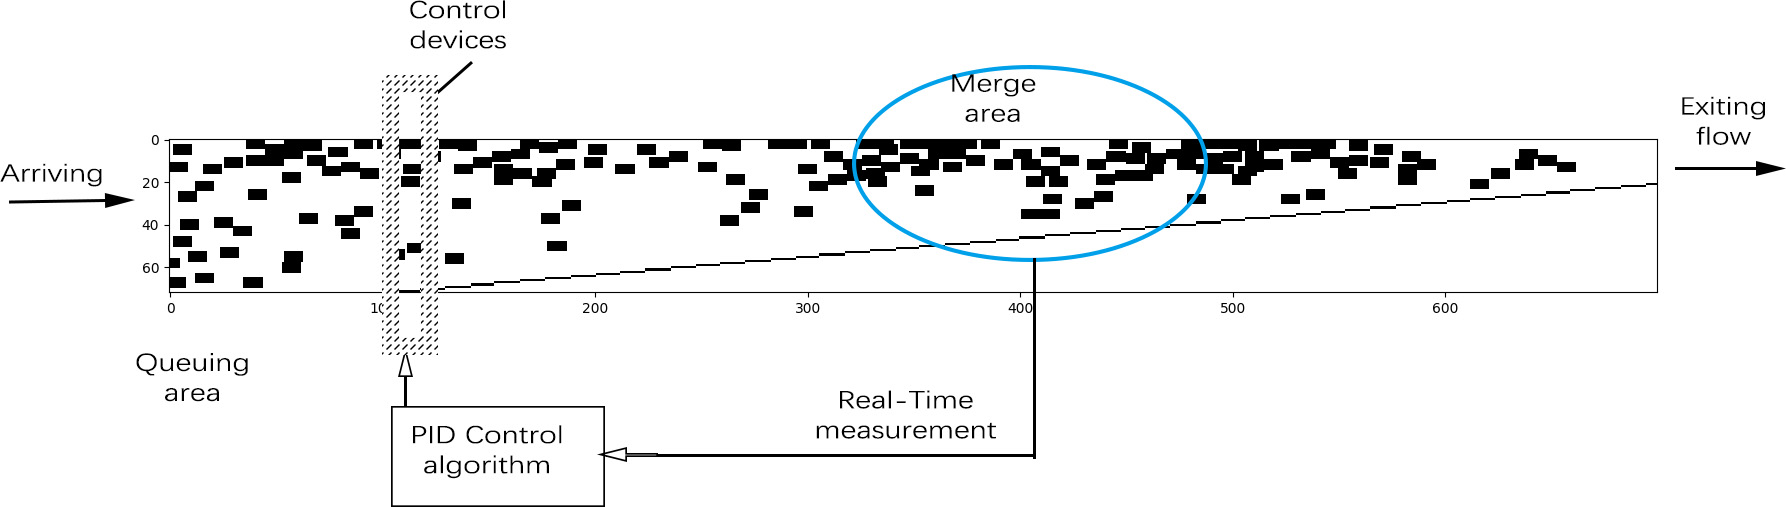
\includegraphics[width=10cm]{figure2}
\caption{The Framework of This System}\label{fig2}
\end{figure}
%此处的figure被放到了下一页

\textbf{Elements}

\textbf{Merge area}

As a matter of fact, the merge area is equal to the
departure zone as referred to above. Typically, it
is an approximately trapezoidal area where the vehicles
leave from the booths on a total of $B$ lanes and finally
fit into $L$ lanes of the exit. Here, we focus on the
flow-density variation with the occupancy increasing
in the merge area. Eventually, we obtain a diagram to
describe this functionary relationship, which is shown
in Figure \ref{fig3}.

\begin{figure}[h]
\small
\centering
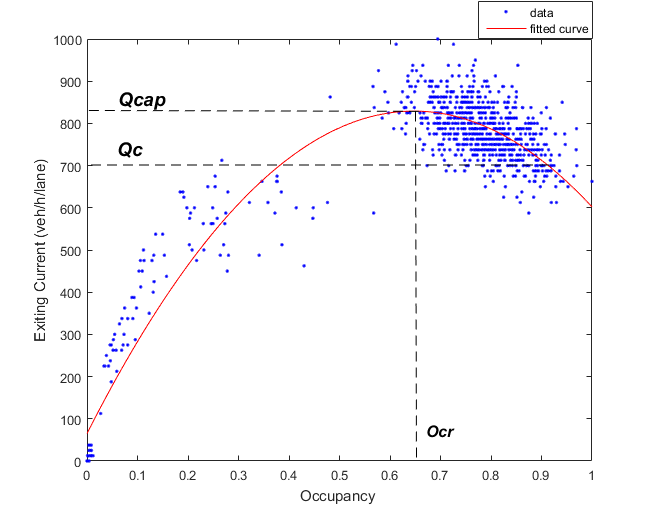
\includegraphics[width=10cm]{figure3}
\caption{The Functionary Relationship}\label{fig3}
\end{figure}

After noticing that X-axis is occupancy $o$ (\%), while
Y-axis represents the exit flow $q_{out}$, we can tell from
the diagram:
\begin{itemize}
\item When $o$ is small, merging conflicts are scarce, and
the exit flow is correspondingly low.
\item As $o$ increases, merging conflicts may increase, but
$q_{out}$ also increases as well until, for a specific value
$o_{cr}$, the exit flow reaches the capacity $q_{cap}$.
\item If $o$ increases beyond $o_{cr}$, merging conflicts
become more frequent, leading to a serious congestion.
Consequently, a capacity drop happens.
\end{itemize}
Therefore, we can conclude that the occupancy of the merge
area can directly influence the exit flow, or rather, the
throughput. And we can regulate the occupancy under the
goal to maintain $o  \approx  o_{cr}$ by controlling the merging
pattern with the assistant of a control algorithm and
feedback. From a macroscopic perspective, the maximum
throughput can be achieved by a certain merging pattern
design. As a result, our goal is to model this design.

\textbf{Feedback control based on ALINEA}

We are inspired by a scheme from a previous article
(\emph{Real-time merging traffic control with applications
to toll plaza and work zone management},2008), and
decide to deploy traffic lights to individual lanes
as control devices.


However, the most crucial task is to determine the
form of feedback control.


We suppose that the feedback control is activated
at each discrete time interval. After activation, it
will collect latest measurements of occupancy $o$, and
send data-converted instructions to control devices
under the purpose of maintaining $o  \approx  o_{cr}$.
Thus, we choose to apply ALINEA as our control algorithm.

ALINEA can be expressed as:

\[q\left( n \right) = q\left( {n - 1} \right) + {K_R}\left[ {\hat{o}  - o(n - 1)} \right]\]

Where,

% Table generated by Excel2LaTeX from sheet 'Sheet1'
\begin{table}[htbp]
  \centering
    \begin{tabular}{ll}
      \toprule
    $n$     & The discrete time index \\
    $q(n)$  & The controlled entering flow (veh/h) to be implemented in a new time step $n$ \\
    $q(n-1)$ & The existed entering flow (veh/h) in last time step \\
    $o(n-1)$ & The measured occupancy of merge area in last time step \\
    $\hat{o}$ & The desired value of occupancy (can be set as $o_{cr}$) \\
    $K_{R}$  & A regulator parameter, always positive \\
    \bottomrule
    \end{tabular}%
  \label{tab:addlabel}%
\end{table}%

In addition, the occupancy measurement should best be
placed at or just upstream of the location where serious
vehicle decelerations (congestion) appear first.

\section{Conclusion}

\section{Sensitivity Analysis}
\subsection{The Performance of Our Solution in Light
and Heavy Traffic}
\subsection{Autonomous Vehicles}
\subsection{The Proportions of Different Tollbooths}

\section{Strengths and Weaknesses}
\subsection{Strengths}
\subsection{Weaknesses}

\begin{thebibliography}{99}
\bibitem{1} D. E. KNUTH   The \TeX{}book  the American
Mathematical Society and Addison-Wesley
Publishing Company , 1984-1986.
\bibitem{2}Lamport, Leslie,  \LaTeX{}: `` A Document Preparation System '',
Addison-Wesley Publishing Company, 1986.

\end{thebibliography}

\begin{appendices}

\section{First appendix}


Here are simulation programmes we used in our model as follow.\\

\textbf{\textcolor[rgb]{0.98,0.00,0.00}{Input matlab source:}}
\lstinputlisting[language=Matlab]{./code/mcmthesis-matlab1.m}

\section{Second appendix}

some more text \textcolor[rgb]{0.98,0.00,0.00}{\textbf{Input C++ source:}}
\lstinputlisting[language=C++]{./code/mcmthesis-sudoku.cpp}

\end{appendices}
\end{document}

%%
%% This work consists of these files mcmthesis.dtx,
%%                                   figures/ and
%%                                   code/,
%% and the derived files             mcmthesis.cls,
%%                                   mcmthesis-demo.tex,
%%                                   README,
%%                                   LICENSE,
%%                                   mcmthesis.pdf and
%%                                   mcmthesis-demo.pdf.
%%
%% End of file `mcmthesis-demo.tex'.
